\documentclass[12pt]{article}
\usepackage{fullpage}
\usepackage{multicol}
\usepackage{graphicx}
\usepackage{fontspec}
\usepackage{amsfonts}
\usepackage{mathrsfs}
\usepackage{graphicx}
\usepackage{setspace}
\doublespacing
\setmainfont{OpenDyslexicAlta}
\newcommand{\blk}{\underline{\hspace{0.5in}}}
\begin{document}
%\maketitle
\center{\section*{Algebra Test 1 Spring 2020}}
\center{\section*{Work in your notebook.  Show all work for credit!}}
%\begin{multicols}{2}
\begin{enumerate}
\item For each of the following statements, say if it is true or false, if false give a counterexample:
\begin{enumerate}
	\item If you have a quarter, then you have 25 cents.
	\item If $x>3$, then $x = 7$. 
\end{enumerate}

\item Verify that the operations shown below inverses:
\begin{enumerate}
	\item $(4 + 7) - 7$
	\item $\left( \sqrt{49} \right)^2$
\end{enumerate}  

\item Solve the equation for $x$:  $-8x = 16$
\item Solve the equation for $x$: $\frac{1}{3} x = 5$
\item Solve the equation for $x$: $6x + 4 = 16$
\item Solve the equation for $x$: $-2x - 3 = 4x - 5$
\item Solve the equation for $x$: $3(2x + 4) = -6 + 12x$

\item You have a 40\% acid solution of 20 liters. How much water should you add to get a 10\% acid solution?

\item Solve for $y$:  $4x + 2y = 8$

\item Which quadrant of the Cartesian coordinate plane contains the point (3, -5)?

\item  Graph two points $A = (5, 2)$ and $B = (-3, 2)$ on the coordinate plane and measure the length of the segment between them.

\item  True or False:  $(2, 8)$ is a solution for $2x + y = 16$

\item Solve for $y$ when $x = -2$ in the equation  $-3x = 2y + 8$

\item  If $f(x) = 3x - 4$, find $f(5)$.

\item If $f(x) = x^2 -x + 1$, find $f(2)$

%\item   Solve the following equation in terms of y.  6 + 2y =  4x

\item For the equation of the line $y=2x-6$ do the following:
\begin{enumerate}
	\item Find the $x$-intercept
	\item Find the $y$-intercept
	\item Plot the graph
\end{enumerate}

\item For the relation given by $\{(0, 2), (1, 3), (4, 5)\}$:
\begin{enumerate}
	\item What is the Domain?
	\item What is the Range?
	\item Is it a function?
\end{enumerate}

\newpage

\item For each of the relations shown below tell me the Domain, Range, and Whether or not it is a function.
\begin{enumerate}
	\item \hspace{0.5in} \newline 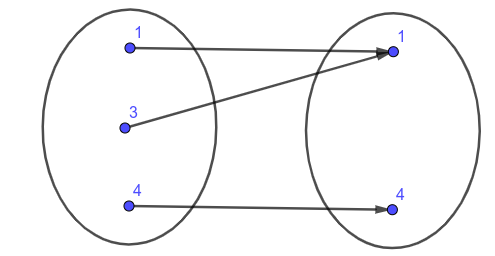
\includegraphics[width=3in]{alg-test3-img1.png}
	\item \hspace{0.5in} \newline 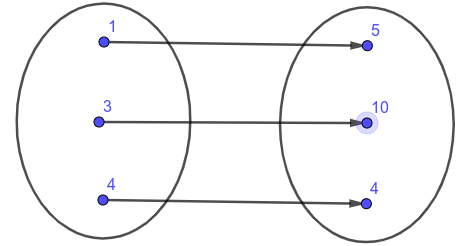
\includegraphics[width=3in]{alg-test3-img2.png}
	\item \hspace{0.5in} \newline 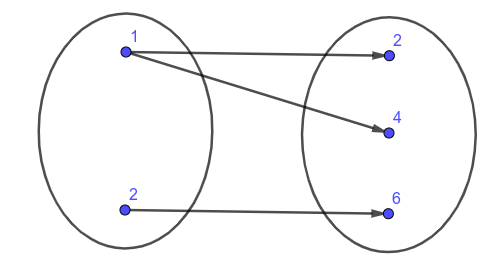
\includegraphics[width=3in]{alg-test3-img3.png}
\end{enumerate}

\item (Extra Credit): Give an example of a line that does not have an \newline $x$-intercept.

\item (Extra Credit): What is the inverse function of the squaring function?
\end{enumerate}
%\end{multicols}
\end{document}